%% Synthesis map (Claude's first draft, 2026-10-21): sources -> themes -> recommendations.
%% Every node and arrow here is a proposal for the researcher to iterate on. Solid arrows: the source directly
%% supports the theme. Dashed: a weaker or interpretive link. Section numbers are live \ref's.
\usetikzlibrary{backgrounds}
\begin{landscape}
\begin{figure}[p]
\centering
\resizebox{\linewidth}{!}{%
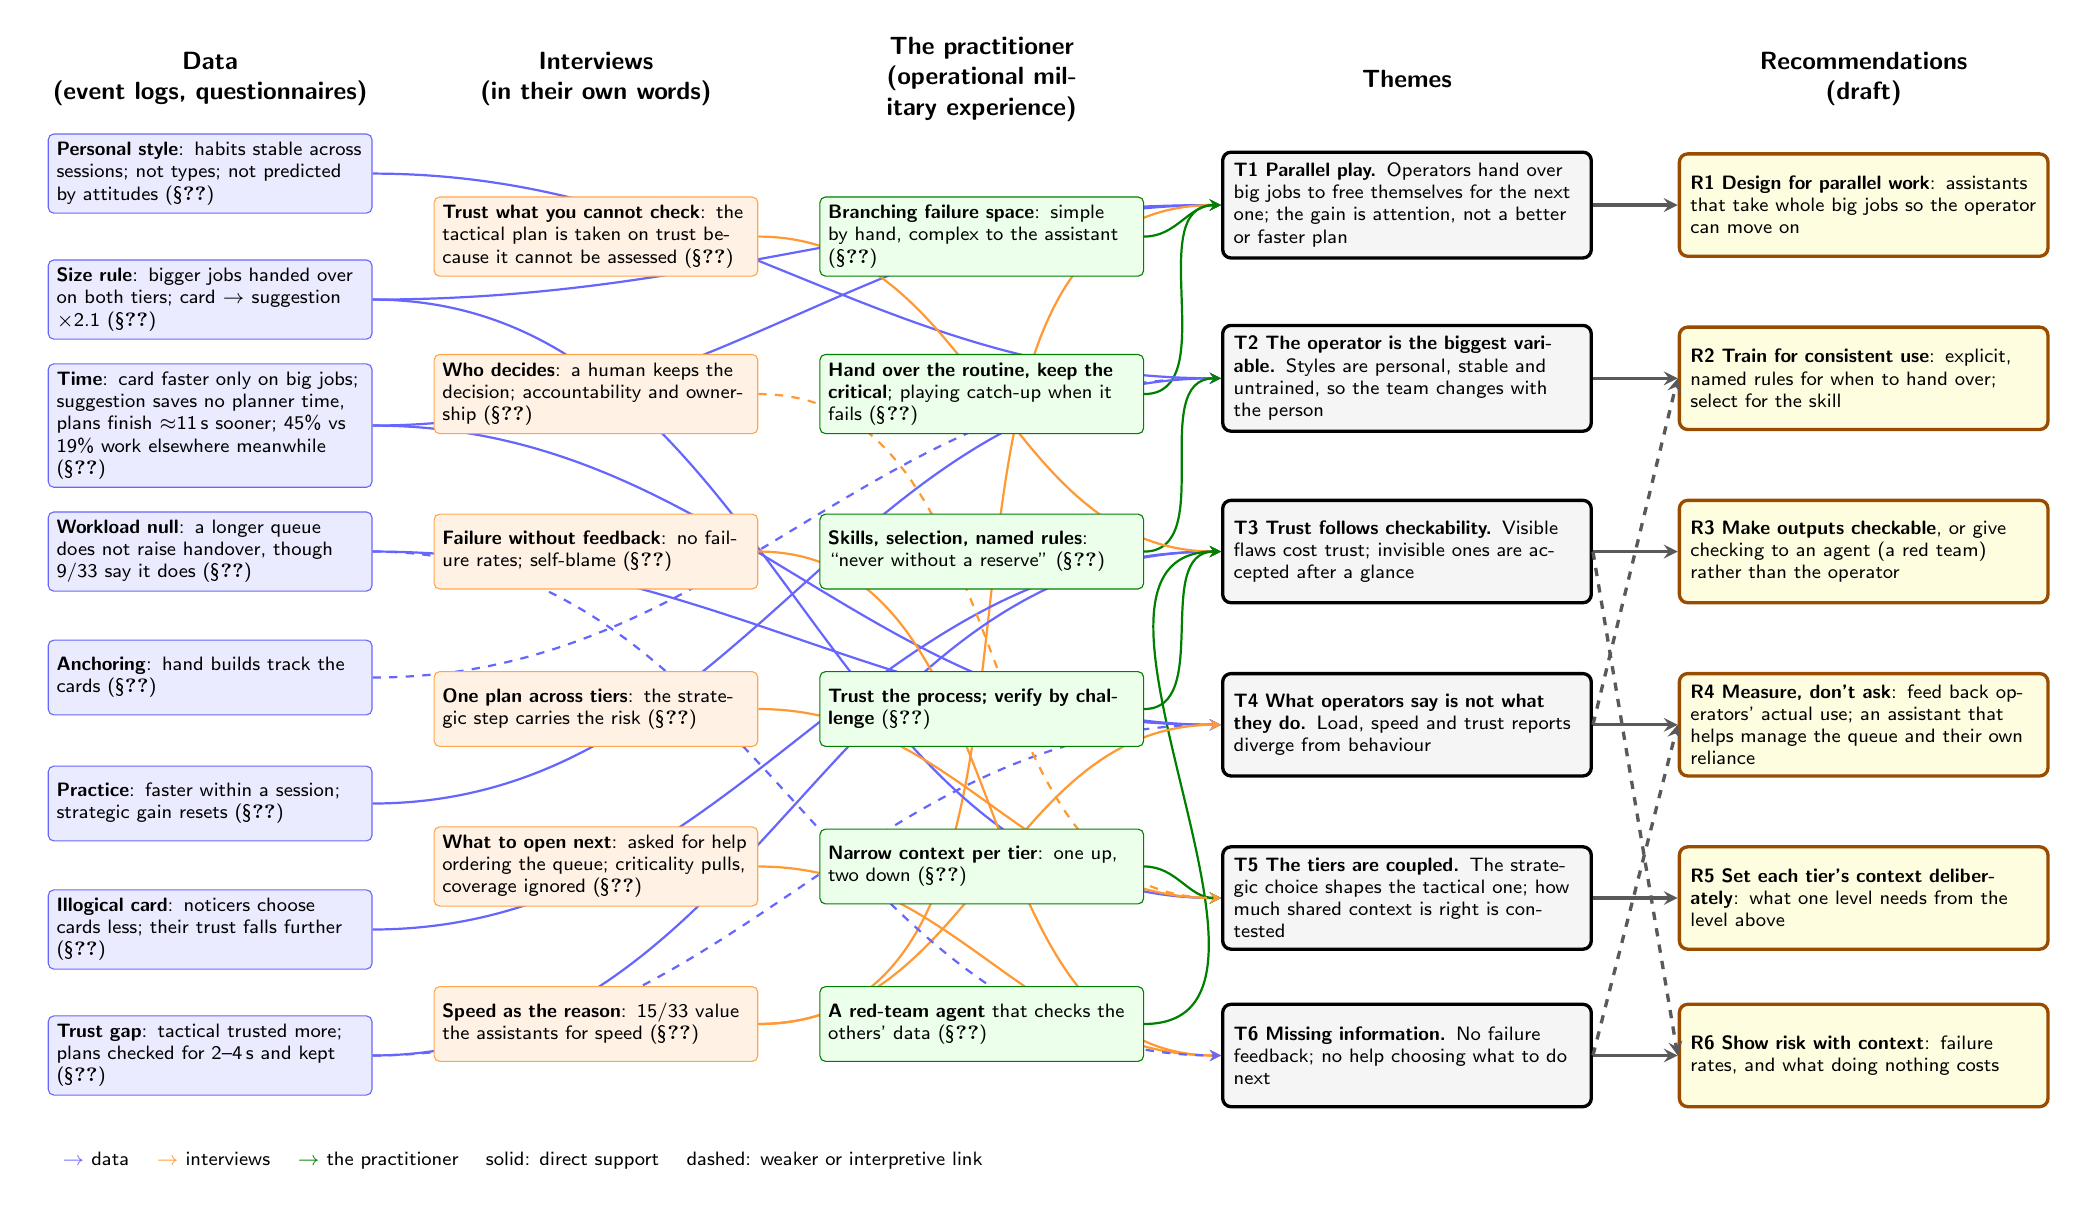
\begin{tikzpicture}[
  font=\sffamily\scriptsize,
  >=stealth,
  src/.style={draw, rounded corners=2pt, align=left, text width=3.9cm, inner sep=3pt, minimum height=0.95cm},
  dat/.style={src, fill=blue!8, draw=blue!60},
  int/.style={src, fill=orange!10, draw=orange!70},
  exp/.style={src, fill=green!8, draw=green!50!black},
  thm/.style={draw, very thick, rounded corners=3pt, align=left, text width=4.4cm, inner sep=4pt, fill=gray!8, minimum height=1.3cm},
  rec/.style={draw, very thick, rounded corners=3pt, align=left, text width=4.4cm, inner sep=4pt, fill=yellow!12, draw=orange!60!black, minimum height=1.3cm},
  ld/.style={->, blue!60, thick},
  li/.style={->, orange!80, thick},
  le/.style={->, green!50!black, thick},
  weak/.style={dashed},
  lt/.style={->, very thick, gray!70!black},
  head/.style={font=\sffamily\small\bfseries, align=center, text width=4.4cm}
]
% ── column headings
\node[head] at (0,1.2) {Data\\(event logs, questionnaires)};
\node[head] at (4.9,1.2) {Interviews\\(in their own words)};
\node[head] at (9.8,1.2) {The practitioner\\(operational military experience)};
\node[head] at (15.2,1.2) {Themes};
\node[head] at (21.0,1.2) {Recommendations\\(draft)};

% ── data findings (x = 0)
\node[dat] (D1) at (0,0)     {\textbf{Personal style}: habits stable across sessions; not types; not predicted by attitudes (\S\ref{sec:res:personal-style})};
\node[dat] (D2) at (0,-1.6)  {\textbf{Size rule}: bigger jobs handed over on both tiers; card $\rightarrow$ suggestion $\times$2.1 (\S\ref{sec:res:size-decides})};
\node[dat] (D3) at (0,-3.2)  {\textbf{Time}: card faster only on big jobs; suggestion saves no planner time, plans finish $\approx$11\,s sooner; 45\% vs 19\% work elsewhere meanwhile (\S\ref{sec:res:size-decides:speed})};
\node[dat] (D4) at (0,-4.8)  {\textbf{Workload null}: a longer queue does not raise handover, though 9/33 say it does (\S\ref{sec:res:workload})};
\node[dat] (D5) at (0,-6.4)  {\textbf{Anchoring}: hand builds track the cards (\S\ref{sec:res:manual-cards})};
\node[dat] (D6) at (0,-8.0)  {\textbf{Practice}: faster within a session; strategic gain resets (\S\ref{sec:res:practice})};
\node[dat] (D7) at (0,-9.6)  {\textbf{Illogical card}: noticers choose cards less; their trust falls further (\S\ref{sec:res:flaw-odd})};
\node[dat] (D8) at (0,-11.2) {\textbf{Trust gap}: tactical trusted more; plans checked for 2--4\,s and kept (\S\ref{sec:res:tier-trust})};

% ── interview themes (x = 4.9)
\node[int] (Q1) at (4.9,-0.8)  {\textbf{Trust what you cannot check}: the tactical plan is taken on trust because it cannot be assessed (\S\ref{sec:qual:trust-unchecked})};
\node[int] (Q2) at (4.9,-2.8)  {\textbf{Who decides}: a human keeps the decision; accountability and ownership (\S\ref{sec:qual:who-decides})};
\node[int] (Q3) at (4.9,-4.8)  {\textbf{Failure without feedback}: no failure rates; self-blame (\S\ref{sec:qual:failure})};
\node[int] (Q4) at (4.9,-6.8)  {\textbf{One plan across tiers}: the strategic step carries the risk (\S\ref{sec:qual:hierarchy})};
\node[int] (Q5) at (4.9,-8.8)  {\textbf{What to open next}: asked for help ordering the queue; criticality pulls, coverage ignored (\S\ref{sec:qual:new-jobs:queue-order})};
\node[int] (Q6) at (4.9,-10.8) {\textbf{Speed as the reason}: 15/33 value the assistants for speed (\S\ref{sec:res:size-decides:parallel})};

% ── the practitioner (x = 9.8)
\node[exp] (E1) at (9.8,-0.8)  {\textbf{Branching failure space}: simple by hand, complex to the assistant (\S\ref{sec:qual:practitioner:pt-branching-paths})};
\node[exp] (E2) at (9.8,-2.8)  {\textbf{Hand over the routine, keep the critical}; playing catch-up when it fails (\S\ref{sec:qual:practitioner:pt-play-catch-up})};
\node[exp] (E3) at (9.8,-4.8)  {\textbf{Skills, selection, named rules}: ``never without a reserve'' (\S\ref{sec:qual:practitioner:pt-reserve})};
\node[exp] (E4) at (9.8,-6.8)  {\textbf{Trust the process; verify by challenge} (\S\ref{sec:qual:practitioner:pt-staff-process})};
\node[exp] (E5) at (9.8,-8.8)  {\textbf{Narrow context per tier}: one up, two down (\S\ref{sec:qual:practitioner:pt-silos})};
\node[exp] (E6) at (9.8,-10.8) {\textbf{A red-team agent} that checks the others' data (\S\ref{sec:qual:practitioner:pt-red-team})};

% ── themes (x = 15.2)
\node[thm] (T1) at (15.2,-0.4)  {\textbf{T1 Parallel play.} Operators hand over big jobs to free themselves for the next one; the gain is attention, not a better or faster plan};
\node[thm] (T2) at (15.2,-2.6)  {\textbf{T2 The operator is the biggest variable.} Styles are personal, stable and untrained, so the team changes with the person};
\node[thm] (T3) at (15.2,-4.8)  {\textbf{T3 Trust follows checkability.} Visible flaws cost trust; invisible ones are accepted after a glance};
\node[thm] (T4) at (15.2,-7.0)  {\textbf{T4 What operators say is not what they do.} Load, speed and trust reports diverge from behaviour};
\node[thm] (T5) at (15.2,-9.2)  {\textbf{T5 The tiers are coupled.} The strategic choice shapes the tactical one; how much shared context is right is contested};
\node[thm] (T6) at (15.2,-11.2) {\textbf{T6 Missing information.} No failure feedback; no help choosing what to do next};

% ── recommendations (x = 21.0)
\node[rec] (R1) at (21.0,-0.4)  {\textbf{R1 Design for parallel work}: assistants that take whole big jobs so the operator can move on};
\node[rec] (R2) at (21.0,-2.6)  {\textbf{R2 Train for consistent use}: explicit, named rules for when to hand over; select for the skill};
\node[rec] (R3) at (21.0,-4.8)  {\textbf{R3 Make outputs checkable}, or give checking to an agent (a red team) rather than the operator};
\node[rec] (R4) at (21.0,-7.0)  {\textbf{R4 Measure, don't ask}: feed back operators' actual use; an assistant that helps manage the queue and their own reliance};
\node[rec] (R5) at (21.0,-9.2)  {\textbf{R5 Set each tier's context deliberately}: what one level needs from the level above};
\node[rec] (R6) at (21.0,-11.2) {\textbf{R6 Show risk with context}: failure rates, and what doing nothing costs};

% ── sources -> themes (solid = direct support, dashed = weaker / interpretive), drawn behind the boxes
\begin{pgfonlayer}{background}
\draw[ld] (D2.east) to[out=0,in=180] (T1.west);
\draw[ld] (D3.east) to[out=0,in=180] (T1.west);
\draw[li] (Q6.east) to[out=0,in=180] (T1.west);
\draw[le] (E1.east) to[out=0,in=180] (T1.west);
\draw[le] (E2.east) to[out=0,in=180] (T1.west);

\draw[ld] (D1.east) to[out=0,in=180] (T2.west);
\draw[ld] (D6.east) to[out=0,in=180] (T2.west);
\draw[ld, weak] (D5.east) to[out=0,in=180] (T2.west);
\draw[le] (E3.east) to[out=0,in=180] (T2.west);

\draw[ld] (D7.east) to[out=0,in=180] (T3.west);
\draw[ld] (D8.east) to[out=0,in=180] (T3.west);
\draw[li] (Q1.east) to[out=0,in=180] (T3.west);
\draw[le] (E4.east) to[out=0,in=180] (T3.west);
\draw[le] (E6.east) to[out=0,in=180] (T3.west);

\draw[ld] (D4.east) to[out=0,in=180] (T4.west);
\draw[ld] (D3.east) to[out=0,in=180] (T4.west);
\draw[ld, weak] (D8.east) to[out=0,in=180] (T4.west);
\draw[li] (Q6.east) to[out=0,in=180] (T4.west);

\draw[ld] (D2.east) to[out=0,in=180] (T5.west);
\draw[li] (Q4.east) to[out=0,in=180] (T5.west);
\draw[le] (E5.east) to[out=0,in=180] (T5.west);
\draw[li, weak] (Q2.east) to[out=0,in=180] (T5.west);

\draw[li] (Q3.east) to[out=0,in=180] (T6.west);
\draw[li] (Q5.east) to[out=0,in=180] (T6.west);
\draw[ld, weak] (D4.east) to[out=0,in=180] (T6.west);

\end{pgfonlayer}

% ── themes -> recommendations
\draw[lt] (T1) -- (R1);
\draw[lt] (T2) -- (R2);
\draw[lt] (T3) -- (R3);
\draw[lt] (T4) -- (R4);
\draw[lt] (T5) -- (R5);
\draw[lt] (T6) -- (R6);
\draw[lt, weak] (T6.east) -- (R4.west);
\draw[lt, weak] (T4.east) -- (R2.west);
\draw[lt, weak] (T3.east) -- (R6.west);

% ── legend
\node[align=left, anchor=north west, font=\sffamily\scriptsize] at (-2.0,-12.3)
  {\textcolor{blue!60}{$\rightarrow$} data \quad \textcolor{orange!80}{$\rightarrow$} interviews \quad \textcolor{green!50!black}{$\rightarrow$} the practitioner \quad
   solid: direct support \quad dashed: weaker or interpretive link};
\end{tikzpicture}}
\caption{{\color{blue}\textbf{From findings to recommendations (draft).} The key results from the logs and questionnaires (left), the interviews (second column) and the practitioner (third) feed six themes, which point to six draft recommendations. Section numbers link to the evidence. A first sketch for iteration.}}
\label{fig:synthesis-map}
\end{figure}
\end{landscape}
